% Capítulo 6: passagem por valor (cópias) e por referência (outro nome).
\documentclass[border=4pt]{standalone}
\usepackage[utf8]{inputenc}
\usepackage[T1]{fontenc}
% Estilo comum dos fluxogramas e diagramas de blocos.
\usepackage{tikz}
\usetikzlibrary{arrows.meta, positioning, calc, shapes.geometric, shapes.misc}
\definecolor{navy}{RGB}{23,45,80}
\definecolor{laranja}{RGB}{250,110,29}
\definecolor{cinzalogo}{RGB}{107,114,126}
\definecolor{azul}{RGB}{205,222,247}
\tikzset{
  base/.style={draw=navy, line width=0.9pt, font=\sffamily\small, align=center, inner sep=4pt},
  terminal/.style={base, rounded rectangle, fill=laranja!45, draw=laranja, minimum width=20mm, minimum height=7mm},
  processo/.style={base, rectangle, fill=laranja!12, minimum width=28mm, minimum height=8mm},
  decisao/.style={base, diamond, aspect=2.2, fill=azul, inner sep=1pt, minimum width=30mm},
  es/.style={base, trapezium, trapezium left angle=72, trapezium right angle=108,
             fill=white, minimum width=26mm, minimum height=8mm, trapezium stretches body},
  fluxo/.style={-{Stealth[length=2.2mm]}, navy, line width=0.9pt},
  rotulo/.style={font=\sffamily\small\bfseries, text=navy},
  legenda/.style={font=\sffamily\scriptsize, text=cinzalogo},
  resposta/.style={font=\sffamily\scriptsize\bfseries, text=navy},
}

\tikzset{
  cx/.style={draw=navy, line width=0.7pt, minimum width=10mm, minimum height=7mm, font=\sffamily\small\bfseries, text=navy},
  nomevar/.style={font=\ttfamily\small, text=navy},
  copia/.style={-{Stealth[length=2mm]}, laranja, line width=0.9pt, dashed},
  ref/.style={-{Stealth[length=2mm]}, navy, line width=0.9pt},
}
\begin{document}
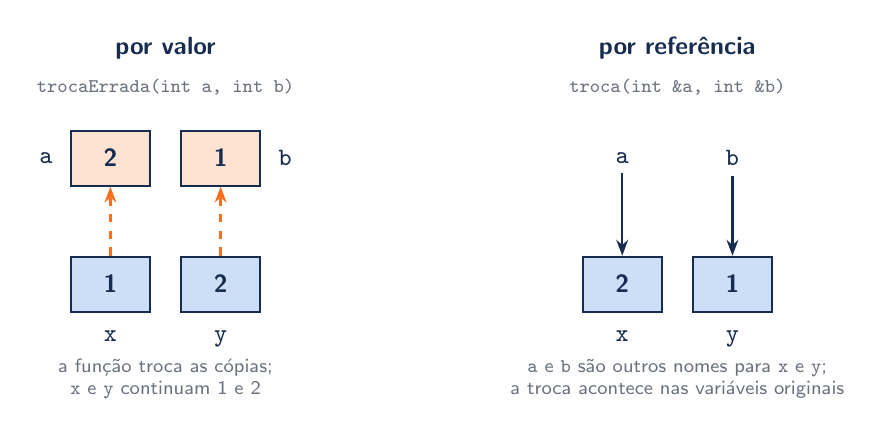
\begin{tikzpicture}
  % por valor
  \node[rotulo] at (0.7, 3.0) {por valor};
  \node[legenda, font=\ttfamily\scriptsize] at (0.7, 2.5) {trocaErrada(int a, int b)};
  \node[cx, fill=azul] (x1) at (0, 0) {1};
  \node[cx, fill=azul] (y1) at (1.4, 0) {2};
  \node[nomevar, below=1mm of x1] {x};
  \node[nomevar, below=1mm of y1] {y};
  \node[cx, fill=laranja!20] (a1) at (0, 1.6) {2};
  \node[cx, fill=laranja!20] (b1) at (1.4, 1.6) {1};
  \node[nomevar, left=1mm of a1] {a};
  \node[nomevar, right=1mm of b1] {b};
  \draw[copia] (x1) -- (a1);
  \draw[copia] (y1) -- (b1);
  \node[legenda, align=center] at (0.7, -1.2) {a função troca as cópias;\\\texttt{x} e \texttt{y} continuam 1 e 2};

  % por referência
  \node[rotulo] at (7.2, 3.0) {por referência};
  \node[legenda, font=\ttfamily\scriptsize] at (7.2, 2.5) {troca(int \&a, int \&b)};
  \node[cx, fill=azul] (x2) at (6.5, 0) {2};
  \node[cx, fill=azul] (y2) at (7.9, 0) {1};
  \node[nomevar, below=1mm of x2] {x};
  \node[nomevar, below=1mm of y2] {y};
  \node[nomevar, font=\ttfamily\small\bfseries] (a2) at (6.5, 1.6) {a};
  \node[nomevar, font=\ttfamily\small\bfseries] (b2) at (7.9, 1.6) {b};
  \draw[ref] (a2) -- (x2);
  \draw[ref] (b2) -- (y2);
  \node[legenda, align=center] at (7.2, -1.2) {\texttt{a} e \texttt{b} são outros nomes para \texttt{x} e \texttt{y};\\a troca acontece nas variáveis originais};
\end{tikzpicture}
\end{document}
